%%%%%%%%%%%%%%%%%%%%%%%%%%%%%%%%%%%%%%%%%
% Lachaise Assignment
% LaTeX Template
% Version 1.0 (26/6/2018)
%
% This template originates from:
% http://www.LaTeXTemplates.com
%
% Authors:
% Marion Lachaise & François Févotte
% Vel (vel@LaTeXTemplates.com)
%
% License:
% CC BY-NC-SA 3.0 (http://creativecommons.org/licenses/by-nc-sa/3.0/)
%
%%%%%%%%%%%%%%%%%%%%%%%%%%%%%%%%%%%%%%%%%

%----------------------------------------------------------------------------------------
%	PACKAGES AND OTHER DOCUMENT CONFIGURATIONS
%----------------------------------------------------------------------------------------

\documentclass{article}

%%%%%%%%%%%%%%%%%%%%%%%%%%%%%%%%%%%%%%%%%
% Lachaise Assignment
% Structure Specification File
% Version 1.0 (26/6/2018)
%
% This template originates from:
% http://www.LaTeXTemplates.com
%
% Authors:
% Marion Lachaise & François Févotte
% Vel (vel@LaTeXTemplates.com)
%
% License:
% CC BY-NC-SA 3.0 (http://creativecommons.org/licenses/by-nc-sa/3.0/)
% 
%%%%%%%%%%%%%%%%%%%%%%%%%%%%%%%%%%%%%%%%%

%----------------------------------------------------------------------------------------
%	PACKAGES AND OTHER DOCUMENT CONFIGURATIONS
%----------------------------------------------------------------------------------------

\usepackage{amsmath,amsfonts,stmaryrd,amssymb} % Math packages

\usepackage{enumerate} % Custom item numbers for enumerations

\usepackage[ruled]{algorithm2e} % Algorithms

\usepackage[framemethod=tikz]{mdframed} % Allows defining custom boxed/framed environments

\usepackage{listings} % File listings, with syntax highlighting
\lstset{
	basicstyle=\ttfamily, % Typeset listings in monospace font
}
\usepackage{subcaption}

%----------------------------------------------------------------------------------------
%	DOCUMENT MARGINS
%----------------------------------------------------------------------------------------

\usepackage{geometry} % Required for adjusting page dimensions and margins

\geometry{
	paper=a4paper, % Paper size, change to letterpaper for US letter size
	top=2.5cm, % Top margin
	bottom=3cm, % Bottom margin
	left=2.5cm, % Left margin
	right=2.5cm, % Right margin
	headheight=14pt, % Header height
	footskip=1.5cm, % Space from the bottom margin to the baseline of the footer
	headsep=1.2cm, % Space from the top margin to the baseline of the header
	%showframe, % Uncomment to show how the type block is set on the page
}

%----------------------------------------------------------------------------------------
%	FONTS
%----------------------------------------------------------------------------------------

\usepackage[utf8]{inputenc} % Required for inputting international characters
\usepackage[T1]{fontenc} % Output font encoding for international characters

\usepackage{XCharter} % Use the XCharter fonts

%----------------------------------------------------------------------------------------
%	COMMAND LINE ENVIRONMENT
%----------------------------------------------------------------------------------------

% Usage:
% \begin{commandline}
%	\begin{verbatim}
%		$ ls
%		
%		Applications	Desktop	...
%	\end{verbatim}
% \end{commandline}

\mdfdefinestyle{commandline}{
	leftmargin=10pt,
	rightmargin=10pt,
	innerleftmargin=15pt,
	middlelinecolor=black!50!white,
	middlelinewidth=2pt,
	frametitlerule=false,
	backgroundcolor=black!5!white,
	frametitle={Command Line},
	frametitlefont={\normalfont\sffamily\color{white}\hspace{-1em}},
	frametitlebackgroundcolor=black!50!white,
	nobreak,
}

% Define a custom environment for command-line snapshots
\newenvironment{commandline}{
	\medskip
	\begin{mdframed}[style=commandline]
}{
	\end{mdframed}
	\medskip
}

%----------------------------------------------------------------------------------------
%	FILE CONTENTS ENVIRONMENT
%----------------------------------------------------------------------------------------

% Usage:
% \begin{file}[optional filename, defaults to "File"]
%	File contents, for example, with a listings environment
% \end{file}

\mdfdefinestyle{file}{
	innertopmargin=1.6\baselineskip,
	innerbottommargin=0.8\baselineskip,
	topline=false, bottomline=false,
	leftline=false, rightline=false,
	leftmargin=2cm,
	rightmargin=2cm,
	singleextra={%
		\draw[fill=black!10!white](P)++(0,-1.2em)rectangle(P-|O);
		\node[anchor=north west]
		at(P-|O){\ttfamily\mdfilename};
		%
		\def\l{3em}
		\draw(O-|P)++(-\l,0)--++(\l,\l)--(P)--(P-|O)--(O)--cycle;
		\draw(O-|P)++(-\l,0)--++(0,\l)--++(\l,0);
	},
	nobreak,
}

% Define a custom environment for file contents
\newenvironment{file}[1][File]{ % Set the default filename to "File"
	\medskip
	\newcommand{\mdfilename}{#1}
	\begin{mdframed}[style=file]
}{
	\end{mdframed}
	\medskip
}

%----------------------------------------------------------------------------------------
%	NUMBERED QUESTIONS ENVIRONMENT
%----------------------------------------------------------------------------------------

% Usage:
% \begin{question}[optional title]
%	Question contents
% \end{question}

\mdfdefinestyle{question}{
	innertopmargin=1.2\baselineskip,
	innerbottommargin=0.8\baselineskip,
	roundcorner=5pt,
	nobreak,
	singleextra={%
		\draw(P-|O)node[xshift=1em,anchor=west,fill=white,draw,rounded corners=5pt]{%
		Question \theQuestion\questionTitle};
	},
}

\newcounter{Question} % Stores the current question number that gets iterated with each new question

% Define a custom environment for numbered questions
\newenvironment{question}[1][\unskip]{
	\bigskip
	\stepcounter{Question}
	\newcommand{\questionTitle}{~#1}
	\begin{mdframed}[style=question]
}{
	\end{mdframed}
	\medskip
}

%----------------------------------------------------------------------------------------
%	WARNING TEXT ENVIRONMENT
%----------------------------------------------------------------------------------------

% Usage:
% \begin{warn}[optional title, defaults to "Warning:"]
%	Contents
% \end{warn}

\mdfdefinestyle{warning}{
	topline=false, bottomline=false,
	leftline=false, rightline=false,
	nobreak,
	singleextra={%
		\draw(P-|O)++(-0.5em,0)node(tmp1){};
		\draw(P-|O)++(0.5em,0)node(tmp2){};
		\fill[black,rotate around={45:(P-|O)}](tmp1)rectangle(tmp2);
		\node at(P-|O){\color{white}\scriptsize\bf !};
		\draw[very thick](P-|O)++(0,-1em)--(O);%--(O-|P);
	}
}

% Define a custom environment for warning text
\newenvironment{warn}[1][Warning:]{ % Set the default warning to "Warning:"
	\medskip
	\begin{mdframed}[style=warning]
		\noindent{\textbf{#1}}
}{
	\end{mdframed}
}

%----------------------------------------------------------------------------------------
%	INFORMATION ENVIRONMENT
%----------------------------------------------------------------------------------------

% Usage:
% \begin{info}[optional title, defaults to "Info:"]
% 	contents
% 	\end{info}

\mdfdefinestyle{info}{%
	topline=false, bottomline=false,
	leftline=false, rightline=false,
	nobreak,
	singleextra={%
		\fill[black](P-|O)circle[radius=0.4em];
		\node at(P-|O){\color{white}\scriptsize\bf i};
		\draw[very thick](P-|O)++(0,-0.8em)--(O);%--(O-|P);
	}
}

% Define a custom environment for information
\newenvironment{info}[1][Info:]{ % Set the default title to "Info:"
	\medskip
	\begin{mdframed}[style=info]
		\noindent{\textbf{#1}}
}{
	\end{mdframed}
}
 % Include the file specifying the document structure and custom commands
%Als we extra packages willen laden kan dat het best in structure.tex


% Define matices for pretty functions
\def\r{
	\begin{pmatrix}
		x \\
		y \\
		z
	\end{pmatrix}}

\def\dr{
	\begin{pmatrix}
		\dot{x} \\
		\dot{y} \\
		\dot{z}
	\end{pmatrix}}

\def\Nabla{
	\begin{pmatrix}
		\frac{\partial}{\partial {x}} \\
		\frac{\partial}{\partial {y}} \\
		\frac{\partial}{\partial {z}}
	\end{pmatrix}}

\def\dNabla{
	\begin{pmatrix}
		\frac{\partial}{\partial \dot{x}} \\
		\frac{\partial}{\partial \dot{y}} \\
		\frac{\partial}{\partial \dot{z}}
	\end{pmatrix}}


\begin{document}

\section{Principle of Fermat}

\textit{\underline{Question:} Proof that equation \ref{eq_1.3} and \ref{eq_1.4} can be reduced to equation \ref{eq_1.6}.} \\

\begin{equation}
	\label{eq_1.3}
	L[x,y,z,\dot{X},\dot{y},\dot{z}] = n(x,y,z)\sqrt{\dot{x}^2+\dot{y}^2+\dot{z}^2}
\end{equation}

\begin{equation}
	\label{eq_1.4}
	\frac{d}{dt} \frac{\partial L}{\partial \dot{x}} - \frac{\partial L}{\partial x} = 0, \frac{d}{dt} \frac{\partial L}{\partial \dot{y}} - \frac{\partial L}{\partial y} = 0, \frac{d}{dt} \frac{\partial L}{\partial \dot{z}} - \frac{\partial L}{\partial z} = 0
\end{equation}

\begin{equation}
	\label{eq_1.6}
	\frac{d}{ds} \left[ n \frac{d \vec{r}}{ds} \right] = \vec{\nabla} n
\end{equation} \\
\textit{\underline{Answer:}}\\
\\
First noting that $ds$ is a small element of distance travelled. Therefore taking into account the $x$, $y$ and $z$ direction, $ds$ is given by: \\

\begin{equation}
	ds = \sqrt{{dx}^2+{dy}^2+{dz}^2}
\end{equation}

A small distance travelled in a trivial direction, lets say $dx$, can be approximated by as $dx = dt \cdot \dot{x}$. Therefore $ds$ can be rewritten as: \\

\begin{equation}
	ds = dt \sqrt{\dot{x}^2+\dot{y}^2+\dot{z}^2}
\end{equation}

Rewriting gives:

\begin{equation}
	\label{eq_dsdt}
	\sqrt{\dot{x}^2+\dot{y}^2+\dot{z}^2} = \frac{ds}{dt}
\end{equation}

If we combine the equations in equation \ref{eq_1.4} in vector notation we get: \\

\begin{equation}
	\frac{d}{dt} \dNabla L - \nabla L = 0
\end{equation}

Rewriting and filling in equation \ref{eq_1.3} gives:

\begin{equation}
	\frac{d}{dt} \left[ \dNabla n(x,y,z)\sqrt{\dot{x}^2+\dot{y}^2+\dot{z}^2} \right] = \Nabla \left[ n(x,y,z)\sqrt{\dot{x}^2+\dot{y}^2+\dot{z}^2} \right]
\end{equation}

\begin{equation}
	\frac{d}{dt}  \frac{n \cdot \dot{\vec{r}} }{\sqrt{\dot{x}^2+\dot{y}^2+\dot{z}^2}}   = \vec{\nabla} n \; \sqrt{\dot{x}^2+\dot{y}^2+\dot{z}^2}
\end{equation}

Using equation \ref{eq_dsdt} to to replace the $\sqrt{\dot{x}^2+\dot{y}^2+\dot{z}^2}$ and rewriting the $\dot{\vec{r}}$ vector gives the following: \\

\begin{equation}
	\frac{d}{dt} \frac{n \cdot \dot{\vec{r}}}{\frac{ds}{dt}}  = \vec{\nabla} n \: \frac{ds}{dt}
\end{equation}

\begin{equation}
	\frac{d}{dt}  \frac{n \cdot \frac{d}{dt} \vec{r}}{\frac{ds}{dt}}   =  \vec{\nabla} n \: \frac{ds}{dt}
\end{equation}

Rewriting yields the equation that was to be proved: \\

\begin{equation}
	\frac{d}{ds} \left[ n \frac{d \vec{r}}{ds} \right] = \vec{\nabla} n
\end{equation}

\section{Application}
\subsection{Homogeneous medium}

\textit{\underline{Question:} Using equation \ref{eq_1.6}, show how light is travelling in a homogeneous medium.}\\
\\
\textit{\underline{Answer:}} \\
\\
Equation \ref{eq_1.6} can be rewritten using the chain rule: \\

\begin{equation}
	\frac{d \vec{r}}{ds} \frac{d}{ds} n + n \frac{d^2 \vec{r}}{ds^2} = \Nabla n
\end{equation} \\

Note that for a homogeneous medium, the index of refraction, $n$, is constant. Therefore $\frac{dn}{ds} = 0$, $\frac{\partial n}{\partial x} = 0$, $\frac{\partial n}{\partial y} = 0$ and $\frac{\partial n}{\partial z} = 0$. Using this in the previous equation yields: \\

\begin{equation}
	 n \frac{d^2 \vec{r}}{ds^2} = \vec{0}
\end{equation}

\begin{equation}
	 \frac{d^2 \vec{r}}{ds^2} = \vec{0}
\end{equation} \\


This implies that the direction and velocity of the light is not changed as the light travels through the medium. Therefore, it travels in a straight line with a constant velocity.\\

\newpage
\subsection{Snell-Descartes Law}

\textit{\underline{Question:} Express first geometrically and then analytically Snell and Descartes law of reflection and transmission of the light at the interface between two media of different index of refraction $n_1$ and $n_2$, using the Principle of Fermat and equation \ref{eq_1.6}.}\\
\\
\textit{\underline{Answer:}} \\
\subsubsection{Geometrical}
The speed of light in a medium is inversely proportional to the refractive index. Therefore, the shortest path (in distance) between two points in materials with different refractive indices is not always the fastest (in time). This phenomenon is nicely described by a 2-dimensional analogy of a beach (see figure \ref{fig_snell_empty}). The maximum speed on foot on beach is significantly higher than the maximum swimming speed in the water. So if somebody would need to get from a point A on the beach to a point B in the water, the direct route from A to B (dashed line in figure \ref{fig_snell_empty}) would intuitively be slower than the path with a shorter swimming distance (solid line in figure \ref{fig_snell_empty}).

\begin{figure}[h!]
	\centering
	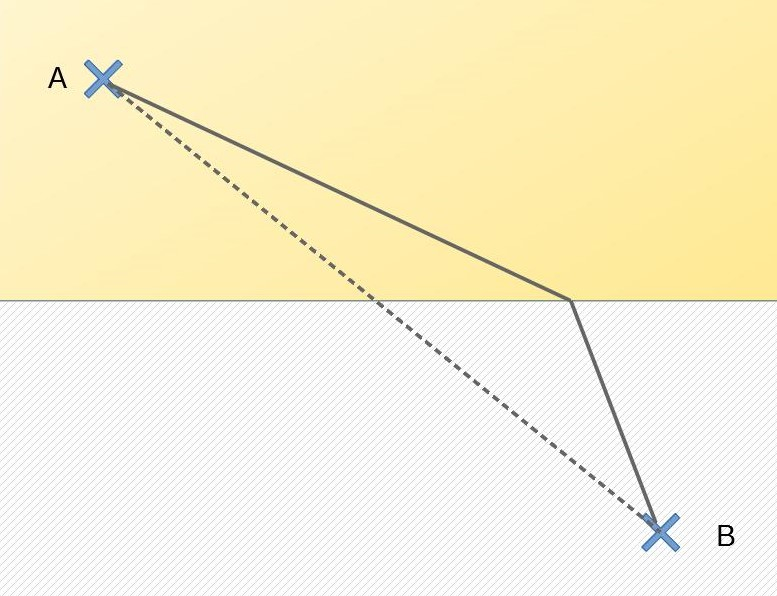
\includegraphics[width=8cm]{afbeeldingen/snell_diagram_leeg.jpg}
	\caption{Diagram of a 2-dimensional beach analogy of the interface between two media with different index of refraction. The upper-half corresponds to the beach and the lower-half to the sea. The dashed line corresponds to the direct route between point A and B with the shortest distance. The solid line corresponds to a route that is intuitively faster than the direct route.}
	\label{fig_snell_empty}
\end{figure}

It is possible to calculate the fastest route between point A and B If we add the parameters $v_1$, $v_2$, $\theta _1$, $\theta _2$, $a$, $b$, $c$ and $d$ which corresponds respectively to the propagation speed on the beach, the propagation speed in the water, the angle of the path on the beach with the normal, the angle of the path in the water with the normal and distances which can be seen in figure \ref{fig_snell_full}.

\begin{figure}[h!]
	\centering
	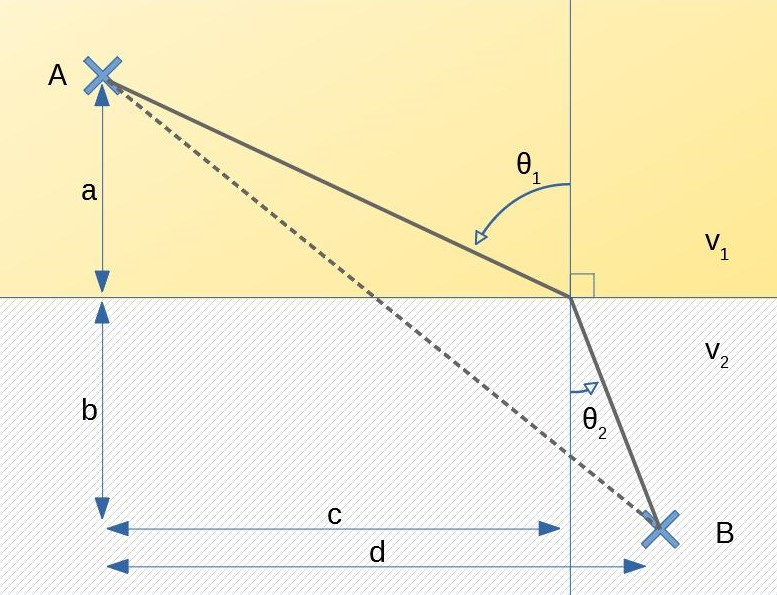
\includegraphics[width=8cm]{afbeeldingen/snell_diagram_vol.jpg}
	\caption{Diagram of beach analogy with parameters $v_1$, $v_2$, $\theta _1$, $\theta _2$, $a$, $b$, $c$ and $d$. These correspond respectively to the propagation speed on the beach, the propagation speed in the water, the angle of the path on the beach with the normal, the angle of the path in the water with the normal and distances which can be seen in the diagram.}
	\label{fig_snell_full}
\end{figure}

The time it takes to travel from point A to B, $t$, can easily be found dividing the path on the beach and the water, respectively $l_{beach}$ and $l_{water}$ by the corresponding speed:

\begin{equation}
	t = l_{beach}/v_1 + l_{water}/v_2
\end{equation}

Using the pythagoras theorem we find:

\begin{equation}
	t = \sqrt{a^2 + c^2}/v_1 + \sqrt{b^2 + (d-c)^2}/v_2
	\label{eq_t}
\end{equation}

If there is a fastest path, there should be an optimum value for $c$ for which $dt/dc = 0$. Therefore, applying the principle of Fermat to equation \ref{eq_t} leads to the following:

\begin{equation}
	0 = \frac{c}{v_1 \sqrt{a^2 + c^2}} + \frac{c-d}{v_2 \sqrt{b^2 + (d-c)^2}}
\end{equation}

We now need the following trigonometric identity for right-angled triangles:
 
\begin{equation}
	sin(\theta) = (adjacent-side)/(diagonal-side) 
	\label{eq_sin_identity}
\end{equation}

Filling in this identity yields:

\begin{equation}
	0 =  sin(\theta _1)/v_1 - sin(\theta _2)/v_2
\end{equation}

If we rewrite this and use the fact that the speed of light in a medium is given by $v = c/n$ we obtain Snell-Descartes law:

\begin{equation}
	n_1 \; sin(\theta _1) = n_2 \; sin(\theta _2)
\end{equation}

This equation basically tells us, that for a interface to a higher refractive index, so where the light slows down, the light bends to the normal.

\subsubsection{Analytical}

For the analytical derivation of Snell-Descartes law we will use a similar diagram as in the geometrical derivation with a coordinate system added as in figure \ref{fig_snell_analytical}.

\begin{figure}[h!]
\centering
  \begin{subfigure}[b]{0.3\textwidth}
    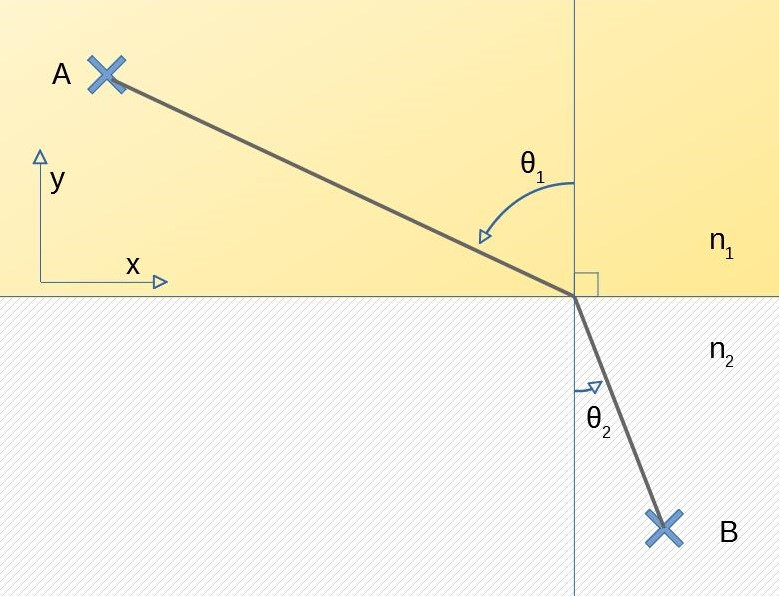
\includegraphics[width=\textwidth]{afbeeldingen/snell_analytical.jpg}
	\caption{Diagram of the path of light at the interface of two media with different refractive indices $n_1$ and $n_2$. $\theta _1$ and $\theta _2$ correspond to the angle with the normal.}
	\label{fig_snell_analytical}
  \end{subfigure}
  \hspace{0.1\textwidth}
  \begin{subfigure}[b]{0.2\textwidth}
    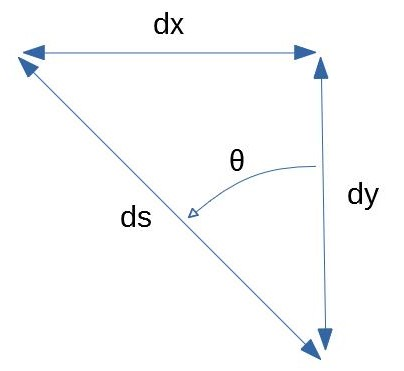
\includegraphics[width=\textwidth]{afbeeldingen/ds.jpg}
	\caption{$ds$ in relation to $dx$ and $dy$.}
	\label{fig_ds}
  \end{subfigure}
  \caption{}
\end{figure}


If we write equation \ref{eq_1.6} for only the x-component and use the fact that $n$ is independent of $x$ in our diagram, we get the following:

\begin{equation}
	\frac{d}{ds} \left[ n \frac{d x}{ds} \right] = \frac{d n}{dx}
\end{equation}

\begin{equation}
	\frac{d}{ds} \left[ n \frac{d x}{ds} \right] = 0
\end{equation}

The $ds$ in the latter equation is defined as in figure \ref{fig_ds}. If we keep a fixed $ds$ for both media we obtain the following equality:

\begin{equation}
	\frac{d}{ds} \left[ n_1 \frac{d x_1}{ds} \right] = \frac{d}{ds} \left[ n_2 \frac{d x_2}{ds} \right]
\end{equation}

Integrating both sides with respect to $ds$ and using the trigonometric identity from equation \ref{eq_sin_identity} yields the Snell-Descartes law:

\begin{equation}
	n_1 \frac{d x_1}{ds}=n_2 \frac{d x_2}{ds}
\end{equation}

\begin{equation}
	n_1 \; sin(\theta _1) = n_2 \; sin(\theta _2)
	\label{eq_snell}
\end{equation}

\newpage
\subsection{Mirage}

\textit{\underline{Question:} The mirage is a common phenomenon when the ground is very warm and the temperature of the air decreases with altitude; in this case the density then increases as well as its index of refraction.\\
\underline{Sketch} what is happening.}\\
\\
\textit{\underline{Answer:}} \\
In figure \ref{fig:mirage} a situation in which a mirage occurs has been sketched. In this figure a few parameters were introduced, an $x$- and $z$-distance respectively denoting the horizontal and vertical distance from the feet of the observer and an angle $\Theta$ which is the angle between the horizontal and the unbent light path from the observer. A gradient effect is also applied to the image, where the colour is darker the index of refraction is higher.\\
Since the index of refraction of the air varies with the temperature and the temperature increases as the $z$-coordinate increases, the path of light rays will be bent. Thus there will be a light ray coming from the sky bending in such a way that it lands in the eye of an observer. This is the mirage effect where light follows a different path than one might expect.\\

\begin{figure}[h!]
	\centering
	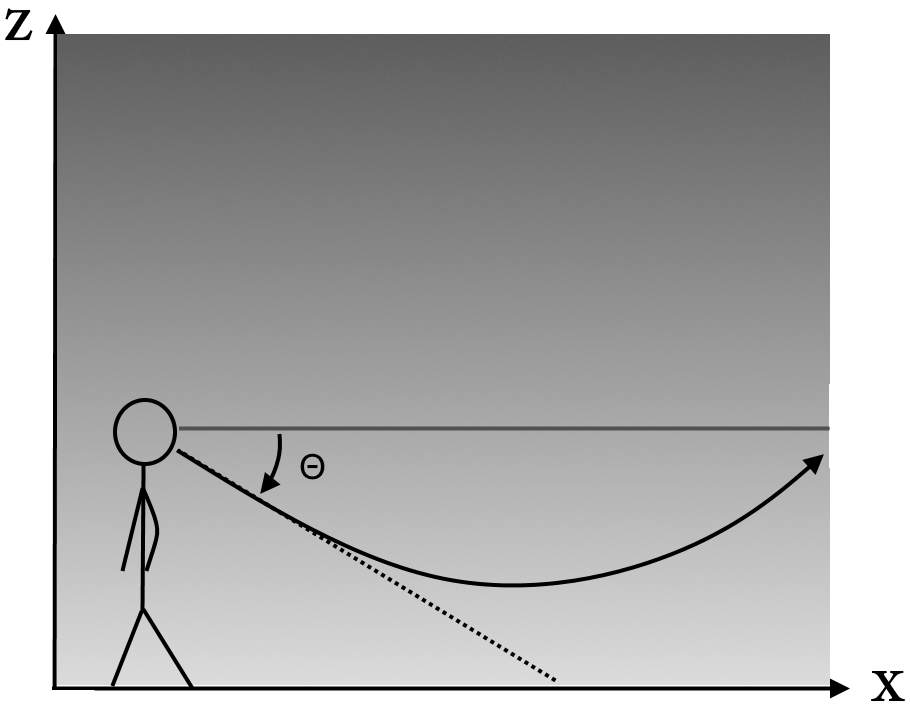
\includegraphics[width=0.4\linewidth,keepaspectratio]{afbeeldingen/miraaj.png}
	\caption{A sketch of situation where a mirage effect occurs.}
	\label{fig:mirage}
\end{figure}
\textit{\underline{Question:} Find the relation between the index of refraction with the altitude if we assume that the gradient of the temperature changes linearly with the altitude.}\\
\\
\textit{\underline{Answer:}} \\
In equation \ref{eq:temp} the temperature at a height $z$ is defined using a ground temperature $T_0$ and a lapse rate $c$ [$K /m$] so that it is linearly decreasing. To relate the index of refraction $n$ to the temperature at height $T(z)$, the Gladstone-Dale relation is used. In equation \ref{eq:glad-dale} this relation is shown with a proportionality constant $K_{air}$. Finally using the equation of state (equation \ref{eq:thermo_formula}), it is possible to relate the index of refraction $n$ to height $z$. Finding the relation for the pressure at height $P(z)$ is shown below in the derivation and the result is displayed in equation \ref{eq:pressure}.\\
\begin{equation}
	T(z) = T_0 - c \cdot z
	\label{eq:temp}
\end{equation}
\begin{equation}
	n-1 \propto K_{air} \rho
	\label{eq:glad-dale}
\end{equation}
\begin{equation}
	\rho = \frac{1}{R_{sp,air}} \frac{P(z)}{T(z)}
	\label{eq:thermo_formula}
\end{equation}
\begin{equation*}
	dT/dz \equiv -c
\end{equation*}
\begin{equation*}
	dP = -g_0 \rho dz
\end{equation*}
\begin{align*}
	dP &= g_0 \frac{\rho}{c} dT\\
	\frac{dP}{P} &= \frac{g_0}{c\cdot R_{sp,air}}\frac{dT}{T}\\
	\int_{P0}^P dP &= \int_{T_0}^T \frac{g_0}{c\cdot R_{sp,air}}\frac{dT}{T}\\
	\ln{P}-\ln{P_0} &= \big[\ln{T} - \ln{T_0}\big] \cdot \frac{g_0}{c\cdot R_{sp,air}}\\
	\frac{P}{P_0} &= (\frac{T}{T_0})^{\frac{g_0}{c\cdot R_{sp,air}}}
\end{align*}
\begin{equation}
	P = P_0 \cdot (\frac{T}{T_0})^{\frac{g_0}{c\cdot R_{sp,air}}}
	\label{eq:pressure}
\end{equation}
After deriving equation \ref{eq:pressure} it is know possible to use both equation \ref{eq:temp} and equation \ref{eq:pressure} to derive the air density $\rho$ with equation \ref{eq:thermo_formula}. The result is show in equation \ref{eq:rho_for_z}, which will be combined with the Gladstone-Dale relation for a equation that equates the index of refraction $n$ with the height $z$. Shown in equation \ref{eq:n_for_z}.\\
\begin{equation*}
	\rho = \frac{P_0}{R_{sp,air}\cdot T(z)} \cdot(\frac{T(z)}{T_0})^{\frac{g_0}{c\cdot R_{sp,air}}}
\end{equation*}
\begin{align*}
	\rho &= \frac{P_0}{R_{sp,air}} \cdot \frac{T(z)^{\frac{g_0}{c R_{sp,air}}}}{T(z)} \cdot (T_0)^{-\frac{g_0}{c R_{sp,air}}}\\
	\rho &= \Bigl[T(z) \Bigr]^{\frac{g_0}{c R_{sp,air}} -1} \frac{P_0}{R_{sp,air}} \cdot T_0^{-\frac{g_0}{c R_{sp,air}}}\\
	\rho &= \Bigl[T_0 -c\cdot z \Bigr]^{\frac{g_0}{c R_{sp,air}} -1} \frac{P_0}{R_{sp,air}} \cdot T_0^{-\frac{g_0}{c R_{sp,air}}}\\
	\rho &= \frac{P_0}{T_0 R_{sp,air}} \Bigl[1-c\cdot z T_0^{-\frac{g_0}{c R_{sp,air}}}\Bigr]
\end{align*}
\begin{equation}
	\rho = \frac{P_0}{T_0 R_{sp,air}} \Bigl[1-c\cdot z T_0^{-\frac{g_0}{c R_{sp,air}}}\Bigr]
	\label{eq:rho_for_z}
\end{equation}
\begin{equation}
	n(z) = K_{air}\rho + 1 = 1 + \frac{P_0 K_{air}}{T_0 R_{sp,air}} \Bigl[1-c\cdot z T_0^{-\frac{g_0}{c R_{sp,air}}}\Bigr]
	\label{eq:n_for_z}
\end{equation}
\textit{\underline{Question:} Express analytically the trajectory of the light in this situation.}\\
\\
\textit{\underline{Answer:}} \\
For an analytical solution it is easier to linearise equation \ref{eq:n_for_z}.
\begin{align*}
	n_l(z) &= n_0 + \alpha \cdot z\\
	n_l(z) &= n(0) +z \cdot \frac{d}{dz}n(z)\rvert_{z=0}
\end{align*}
To get to an analytical solution; equation \ref{eq_1.6} needs to be solved. This is done below.
\begin{equation*}
	\vec{\nabla} \cdot n(z) = \frac{\partial}{\partial z}n(z)= \alpha \vec{e}_z
\end{equation*}
\begin{align*}
	\frac{d}{ds} \Bigl[n(z)\frac{d\vec{r}}{ds}\Bigr] = \vec{\nabla}\cdot n(z) &= \alpha \vec{e}_z\\
	\frac{d}{ds} \Bigl[n(z)\frac{d\vec{x}+d\vec{z}}{\sqrt{dx^2 + dz^2}}\Bigr] &= \alpha \vec{e}_z\\
	\frac{d}{ds} \Bigl[n(z)\frac{dx}{\sqrt{dx^2 + dz^2}}\Bigr] &= 0\\
	\frac{d}{ds} \Bigl[n(z)\frac{dz}{\sqrt{dx^2 + dz^2}}\Bigr] &= \alpha\\
\end{align*}

\begin{align*}
	n(z)\cdot \frac{dx}{\sqrt{dx^2 + dy^2}} &= c\\
	n(z)^2 \cdot \frac{dx^2}{dx^2 + dy^2} &= c^2\\
	n(z)^2 \cdot dx^2 &= c^2(dx^2 + dy^2)\\
	\frac{dz}{dx} = \frac{\sqrt{n(z)^2 -c^2}}{c} &= \frac{\sqrt{(n_0+\alpha\cdot z)^2 -c^2}}{c}
\end{align*}
The above first-order non-linear ordinary differential equation has been solved using wolfram and is displayed below in equation \ref{eq:magic_wolfram}. In this equation, $k$ is an arbitrary constant and $c$ is the total path length. $\alpha$ is the defined linearisation constant.
\begin{equation}
	z(x)=-\frac{c^2 \exp{(\alpha x + \alpha k)/c}+\exp{-(\alpha x + \alpha k)/c}-2n_0}{2 \alpha}
	\label{eq:magic_wolfram}
\end{equation}
\textit{\underline{Question:} Plot several of these trajectories for different relevant cases.}\\
\\
\textit{\underline{Answer:}} \\
Below in figure \ref{fig:paths} a few trajectories for different $\alpha$-values are plotted. These values range from $\alpha = 7.77 \cdot 10^{-7}$ the linearisation constant equal to $d/dz \cdot n(z)\rvert_{z=0}$ to the same constant a magnitude larger.\\

\begin{figure}[h!]
	\centering
	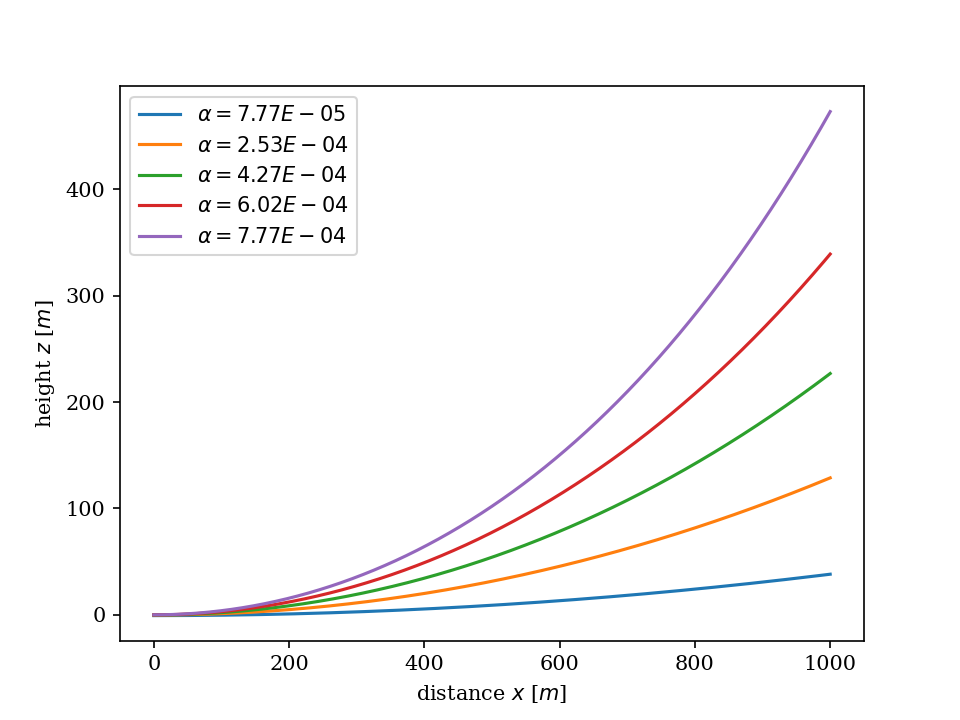
\includegraphics[width=0.5\linewidth,keepaspectratio]{afbeeldingen/light path.png}
	\label{fig:paths}
\end{figure}

\textit{\underline{Question:} Find the closest distance from an observer where a mirage can be visible.}\\
\\
\textit{\underline{Answer:}} \\
In the figure above an $\alpha$-value was used, this value was equal to the derivative of our index of refraction function $n(z)$ evaluated at $x=0$. This value was dependant on the ground temperature $T_0$, the ground pressure $P_0$ and the lapse rate of the temperature $c$. For these the following values were used: $T_0$ $=$ $323.15$ $K$, $P_0$ $=$ $101325$ $Pa$, a lapse rate of $c$ $=$ $1$ $K/m$ and an initial angle of looking down $\theta$ $=$ $15$ degrees. With these conditions you would see the mirage about 500 $m$ in front of you.\\

\textit{\underline{Question:} Forsee what could happen on the north pole when a warm wind is present.}\\
\\
\textit{\underline{Answer:}} \\
On the North Pole with a warm wind blowing an inverse effect as described before would be seen, since the ground is cold and the air heats up as the height increases. The index of refraction $n$ would then decrease the higher off the ground. Light would then bend downward instead of up allowing you to see the ground when you look at the sky.

\subsection{Optical fibre}

\subsubsection{}

\textit{\underline{Question:} If we assume an incoming beam in the $\vartheta _{x,y}$ plane at start crossing $\vartheta _x$ with an angle $\theta _0$. Show that the light beam will stay in this plane and that, by solving the Euler-Lagrange equation \ref{eq_1.6}, the equation for the beam path can be written as:}\\
\begin{equation}
	n \; sin(i) = a
	\label{eq_2.1}
\end{equation}
\\
\textit{\underline{Answer:}} \\
\\

For this question it is assumed that the optical fibre is cylindrical with its axis $\vartheta _x$ (see figure \ref{fig_fibre_3d}). The incident-surface will therefore be in the $\vartheta _{y,z}$ plane.\\

\begin{figure}[h!]
	\centering
	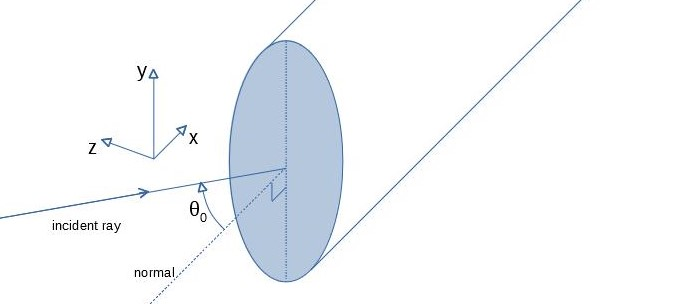
\includegraphics[width=7cm]{afbeeldingen/fibre_3d.jpg}
	\caption{3-dimensional diagram of fibre with incoming light beam making an angle $\theta _0$ with the $\vartheta _x$ axis.}
	\label{fig_fibre_3d}
\end{figure}

When the incoming beam is in the $\vartheta _{x,y}$ plane, the angle with the normal is $\theta _0$ with $\vartheta _x$ in the $\vartheta _y$ direction and $\theta _z = 0$ in the $\vartheta _z$ direction. If we use Snell-Descartes law (equation \ref{eq_snell}) for $\theta _z$ with $\theta _{z,1} = 0$ we obtain $\theta _{z,2} = k \cdot \pi \; [rad]$, with $k = -1,0,1,2,...$. Therefore, the beam of light will stay in the $\vartheta _{x,y}$ plane at the interface, when entering the optical fibre. \\
It is the property of a cylinder that the outer surface is always perpendicular with the radius. For this light beam. Since the light beam is travelling in the $\vartheta _{x,y}$ direction, the outer surface it reaches will be in the $\vartheta _{x,z}$ plane. The angle with the surface normal in the $\vartheta _z$ axis is still zero. From the internal reflection it follows that the angle in  the $\vartheta _z$ axis will remain zero. Therefore, for every reflection at the outer surface, the beam will stay in the $\vartheta _{x,y}$ plane.\\
\\ 
Since we know that the beam will stay in the $\vartheta _{x,y}$ plane, the problem can  be simplified to a 2-dimensional problem (see figure \ref{fig_fibre_2d}). The infinitely small segment $ds$ is related to $ds$, $dy$, $dx$ and $i$ as in figure \ref{fig_fibre_2d}. 

\begin{figure}[h!]
	\centering
	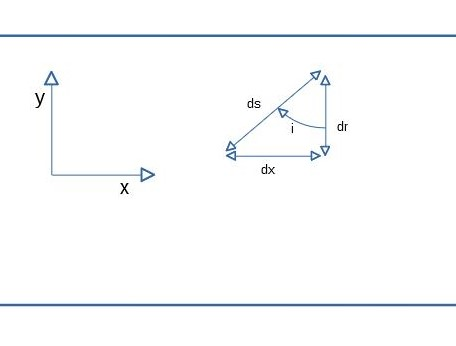
\includegraphics[width = 5cm]{afbeeldingen/fibre_2d.jpg}
	\caption{2-dimensional fibre including the relation between $ds$, $ds$, $dy$, $dx$ and $i$.}
	\label{fig_fibre_2d}
\end{figure}

We can write equtaion \ref{eq_1.6} for only the x-component and use that $n$ is independent of $x$:

\begin{equation}
	\frac{d}{ds} \left[ n \frac{d x}{ds} \right] = \frac{d n}{dx}
\end{equation}

\begin{equation}
	\frac{d}{ds} \left[ n \frac{d x}{ds} \right] = 0
\end{equation}

If we now integrate with respect to $ds$ on both sides we get the following:

\begin{equation}
	n \frac{d x}{ds} = a
\end{equation}

With $a$ an arbitrary constant. From  equation \ref{eq_sin_identity} it follows that $sin(i) = dx/ds$. Using this, we obtain the requested equation:

\begin{equation}
	n \; sin(i) = a
\end{equation}

\subsubsection{}

\textit{\underline{Question:} Solve equation \ref{eq_2.1} for $n(r) = n_0 \sqrt{1 - \alpha ^2 r^2}$ with $\alpha < 1/r$ a constant and $r$ the radius of the fibre.You should end up with an analytical function.}\\
\\
\textit{\underline{Answer:}} \\
From figure \ref{fig_fibre_2d} and equation \ref{eq_sin_identity} it follows that $ sin(i) = dx/ds$. Using this and the Pythagoras theorem in equation \ref{eq_2.1} yields:

\begin{equation*}
	n  \frac{dx}{\sqrt{dr^2 + dx^2}} = a
\end{equation*}

Filling in $n(r)$ and some rewriting results in the following:

\begin{equation*}
	n_0 \sqrt{1 - \alpha ^2 r^2}  \frac{dx}{\sqrt{dr^2 + dx^2}} = a
\end{equation*}

\begin{equation*}
	n_0^2 (1 - \alpha ^2 r^2)  \frac{dx^2}{dr^2 + dx^2} = a^2
\end{equation*}

\begin{equation*}
	n_0^2 (1 - \alpha ^2 r^2)  dx^2 = a^2 (dr^2 + dx^2)
\end{equation*}

\begin{equation*}
	(n_0 ^2 - n_0^2 \alpha ^2 r^2 - a^2)  dx^2 = a^2 dr^2
\end{equation*}

\begin{equation*}
	dx^2 =\frac{a^2 dr^2}{n_0 ^2 - n_0^2 \alpha ^2 r^2 - a^2}
\end{equation*}

\begin{equation*}
	dx =\frac{a \; dr}{\sqrt{n_0 ^2 - n_0^2 \alpha ^2 r^2 - a^2}}
\end{equation*}

If we now integrate both sides we will get:

\begin{equation*}
	\int dx = \int \frac{a}{\sqrt{n_0 ^2 - n_0^2 \alpha ^2 r^2 - a^2}} dr
\end{equation*}

\begin{equation*}
	x = \frac{a}{\sqrt{n_0^2 - a^2}} \int \frac{1}{1 - \left( \frac{r n_0 \alpha}{\sqrt{n_0^2-a^2}} \right) ^2} dr
\end{equation*}

To solve this integral we need the following substitution:

\begin{equation*}
	 \frac{r \; n_0 \; \alpha}{\sqrt{n_0^2-a^2}} = sin(u)
\end{equation*}

\begin{equation*}
	 dr = \frac{\sqrt{n_0^2-a^2}}{n_0 \alpha} cos(u) du
\end{equation*} 

\begin{equation*}
	 u = arcsin \left( \frac{r n_0 \alpha}{\sqrt{n_0^2-a^2}} \right)
\end{equation*}

Using the substitution we get:

\begin{equation*}
	x = \frac{a}{n_0 \; \alpha} \int \frac{\cos (u)}{\sqrt{1 - \sin^2 (u)}} du
\end{equation*}

If we use that $1 - \sin^2 (x) = \cos^2 (x)$, we obtain:

\begin{equation*}
	x = \frac{a}{n_0 \; \alpha} \int \frac{\cos (u)}{\sqrt{\cos^2 (u)}} du
\end{equation*}

\begin{equation*}
	x = \frac{a}{n_0 \; \alpha} \int du
\end{equation*}

\begin{equation*}
	x = \frac{a}{n_0 \; \alpha} u
\end{equation*}

Inverting the substitution and doing some rewriting yields the following equation:

\begin{equation*}
	x = \frac{a}{n_0 \; \alpha} arcsin \left( \frac{r \; n_0 \; \alpha}{\sqrt{n_0^2-a^2}} \right)
\end{equation*}

\begin{equation*}
	\sin \left( \frac{n_0 \; \alpha \; x}{a} \right) =  \frac{r n_0 \alpha}{\sqrt{n_0^2-a^2}}
\end{equation*}

\begin{equation*}
	r(x) = \frac{\sqrt{n_0^2-a^2}}{n_0 \alpha} \sin \left( \frac{n_0 \; \alpha \; x}{a} \right) 
\end{equation*}

Since there are no discontinuities in $n(r)$ and $dn(r)/dr$, we would expect that there are also no discontinuities in $r(x)$ and $dr(x)/dx$. Since $r = \mid y \mid$ for the light beam in the $\vartheta _{x,y}$ plane. The only possible solution of $y(x)$ is the following:

\begin{equation}
	y(x) = \pm \frac{\sqrt{n_0^2-a^2}}{n_0 \alpha} \sin \left( \frac{n_0 \; \alpha \; x}{a}\right) 
\end{equation}



\end{document}
